%%%%%%%%%%%%%%%%%%%%%%%%%%%%%%%%%%%%%%%%%
% Journal Article
% LaTeX Template
% Version 2.0 (February 7, 2023)
%
% This template originates from:
% https://www.LaTeXTemplates.com
%
% Author:
% Vel (vel@latextemplates.com)
%
% License:
% CC BY-NC-SA 4.0 (https://creativecommons.org/licenses/by-nc-sa/4.0/)
%
% NOTE: The bibliography needs to be compiled using the biber engine.
%
%%%%%%%%%%%%%%%%%%%%%%%%%%%%%%%%%%%%%%%%%

%----------------------------------------------------------------------------------------
%	PACKAGES AND OTHER DOCUMENT CONFIGURATIONS
%----------------------------------------------------------------------------------------

\documentclass[
	a4paper, % Paper size, use either a4paper or letterpaper
	10pt, % Default font size, can also use 11pt or 12pt, although this is not recommended
	unnumberedsections, % Comment to enable section numbering
	twoside, % Two side traditional mode where headers and footers change between odd and even pages, comment this option to make them fixed
]{LTJournalArticle}

\usepackage{subcaption}
\usepackage{graphicx}

\addbibresource{references.bib} % BibLaTeX bibliography file

\newcommand{\monthyear}{\ifcase \month \or January\or February\or March\or %
April\or May \or June\or July\or August\or September\or October\or November\or %
December\fi~\number \year}

\setcounter{page}{1} % The page number of the first page, set this to a higher number if the article is to be part of an issue or larger work

%----------------------------------------------------------------------------------------
%	TITLE SECTION
%----------------------------------------------------------------------------------------

\title{Quantifying evolution of service coverage \\ for CIPM MRA participants}


\author{%
	Annette Koo, Joseph Borbely\\ \monthyear
}


\date{Measurement Standards Laboratory of New Zealand, Lower Hutt, New Zealand}

% Full-width abstract
\renewcommand{\maketitlehookd}{%
	\begin{abstract}
		\noindent The key comparison database (KCDB) holds a record of the calibration and measurement capabilities (CMCs) demonstrated by each participant of the CIPM MRA. The total number of CMCs published for a given participant is an often-used but non-discerning measure of the breadth of services maintained by that participant. But now, with the advent of the API to interrogate the KCDB, more nuanced and meaningful measures of service provision can be easily obtained. Here we present an approach, for the Physics domain of the KCDB, to count the number of service categories for which a participant has a CMC in each of the 7 areas within it. We also obtain the evolution of this count with time, benchmarked against other participants.
	\end{abstract}
}

%----------------------------------------------------------------------------------------

\begin{document}

\maketitle % Output the title section


\section{Introduction}

The Mutual Recognition Arrangement of the International Committee for Weights and Measures (CIPM-MRA) is the framework through which participants in the MRA "demonstrate the international equivalence of their measurement standards and mutual acceptance of the calibration and measurement certificates they issue" \cite{CIPMMRAweb}. One of the outcomes of the Arrangement is "the internationally recognized Calibration and Measurement Capabilities (CMCs) of the participating institutes" \cite{CIPMMRAweb}. The peer review of evidence for each capability and the approval of CMCs for publication is carried out in accordance with the requirements of the Arrangement and is administered by the relevant CIPM Consultative Committee for each technical area in partnership with the regional metrology organisations.

It is the responsibility of these committees not only to review evidence and approve claims, but also to maintain a classification of services \cite{Classifications} for which claims can be made. These classifications  are structured in ways that reflect technical distinctions relevant to their area. The KCDB covers three metrology domains: Physics, Chemistry and Biology, and Ionising Radiation. In this work only the Physics domain was considered, so from here on, the discussion will only apply to that domain.

Any participant in the CIPM MRA may claim a CMC for any of the 'individual services' listed by one of the seven areas within the Physics domain: Acoustics, Ultrasound and Vibration; Electricity and Magnetism; Length; Mass and Related Quantities; Photometry and Radiometry; Thermometry; Time and Frequency. The hierarchy of the classification within one of these areas is:

\quad{branch}

\quad{\quad{service}}

\quad{\quad{\quad{sub-service}}}

\quad{\quad{\quad{\quad{individual service}}}}
\vspace{5pt}

For example, within the Mass and Related Quantities area, the first two branches have this structure:

\vspace{5pt}
\quad{BRANCH: Mass}

\quad{\quad{1. Mass}}

\quad{\quad{\quad{1.1 Mass standard}}}

\quad{\quad{\quad{\quad{1.1.1 Mass standard}}}}

\quad{BRANCH: Density}

\quad{\quad{2. Density}}

\quad{\quad{\quad{2.1 Density of solid}}}

\quad{\quad{\quad{\quad{2.1.1 Density of solid}}}}

\quad{\quad{\quad{\quad{2.1.2 Volume of solid}}}}

\quad{\quad{\quad{2.2 Density of liquid}}}

\quad{\quad{\quad{\quad{2.2.1 Density of measuring device}}}}

\quad{\quad{\quad{\quad{2.2.2 Density of liquid}}}}

\quad{\quad{\quad{2.3 Refractive index of liquid}}}

\quad{\quad{\quad{\quad{2.3.1 Refrative index of measuring device}}}}
\vspace{5pt}

In the first branch, Mass, there is only one unique service -- 1.1.1. On the other hand, in the second branch, Density, there are five unique possible services that a participant may claim.

A participant may claim several CMCs within a single individual service category if the uncertainty claim varies with the value measured or with relevant parameters of measurement. It is difficult, therefore, to make meaningful comparisons between participants based simply on the number of CMCs. For example, in response to the MRA review \cite{MRAReview}, the Electricity and Magnetism area collapsed the number of CMCs in the database through the use of a matrix approach to express uncertainties. This reduction in number of CMCs did not reflect a reduction in the range of services available. However, that number is often used as an expression of the breadth of activity and capability of a participant due to the ease of accessing it.

The development of the KCDB API~\cite{KCDBapi} provides a tool for a more sophisticated search and analysis of claims held in the database. One level of sophistication better than the simple number of CMCs claimed is the number of different service categories a participant has claims for. Within the Physics domain, this number can be broken down by area, and within an area, by branch. We describe here how we used the KCDB API and the SI reference point to obtain datasets that were then analysed to deliver this metric. We also make available visual representations of the results.

Note that participation in the CIPM MRA is open to National Metrology Institutes (NMIs) and Designated Institutes (DIs) of Member States of the Metre Convention, of Associate States and Economies, and to certain international organisations invited by the CIPM. In the rest of the paper, we use the term 'participant' to refer to the State, Economy or international organisation rather than the individual NMI or DI; i.e., we count claims by State, Economy or international organisation rather than by NMI or DI.

%------------------------------------------------

\section{KCDB API}

A Python package~\cite{MSLKCDB} was developed to help search the KCDB API for the latest CMCs of each participant. The package provides the option to perform a quick search and an advanced search of all three metrology domains as well as accessing reference data that may be used to filter CMC queries.

\section{Comparative box plots}

Scripts were written to extract the number of unique individual service categories each participant in the CIPM MRA had claims for across each branch of each area in the Physics domain of the KCDB. This number, rather than the raw number of CMCs in each branch, is a better indicator of the breadth of service made available by that participant compared to others.

To visualise this, we generated comparative box and whisker plots comparing the distribution of individual service categories claimed by all MRA participants (with boxes drawn between the first and third quartiles, a line drawn at the median, and whiskers drawn to the 0th and 100th percentile). Any specific participant's data point could then be overlaid on each box.

For example, we show the distribution of service categories across the seven Physics areas in figure \ref{fig:physics_all_nz} with the result for New Zealand overlaid as at December 2024.
The abbreviations used for the areas in the figure are: Acoustics, Ultrasound and Vibration (AUV), Electricity and Magnetism (EM), Length (L), Mass and Related Quantities (M), Photometry and Radiometry (PR), Thermometry (T), Time and Frequency (TF).

\begin{figure}[!htpb]
    \centering
    \includegraphics[width=\linewidth]{../output/box_plots/physics/All/2024/New Zealand.png}
    \caption{Distribution of service categories claimed across the Physics areas in 2024 by all MRA participants (with whiskers drawn to the 0th and 100th percentile) with New Zealand's data overlaid.}
    \label{fig:physics_all_nz}
\end{figure}
We can compare the results of a given participant with any cohort of other participants. Using data extracted from the KCDB in December 2024, we selected participants who have CMCs in at least six of the seven areas of Physics. These participants could be considered to have a broad range of metrological expertise and are therefore dubbed 'Broad range' participants.
We found this 'Broad range' cohort to contain 43 participants, which were Argentina, Australia, Austria, Belarus, Brazil, Bulgaria, Canada, China, Chinese Taipei, Czechia, Denmark, Egypt, Finland, France, Germany, Hong Kong--China, Hungary, Indonesia, Ireland, Italy, Japan, Kazakhstan, Republic of Korea, Malaysia, Mexico, Netherlands, New Zealand, Poland, Portugal, Romania, Russian Federation, Serbia, Singapore, Slovakia, South Africa, Spain, Sweden, Switzerland, Thailand, Turkiye, Ukraine, United Kingdom, and United States.
In figure \ref{fig:physics_broad_nz} we show the distribution of claims for this cohort of participants, again with the results for New Zealand overlaid.

\begin{figure}[!htpb]
    \centering
    \includegraphics[width=\linewidth]{../output/box_plots/physics/Broad/2024/New Zealand.png}
    \caption{Distribution of service categories claimed across the Physics areas in 2024 by 'Broad range' MRA participants (with whiskers drawn to the 0th and 100th percentile) with New Zealand's data overlaid.}
    \label{fig:physics_broad_nz}
\end{figure}

\section{Evolution of service coverage}

Looking at the history of current CMC claims, we can gain insight into the evolution over time of the claims in the KCDB and also of the claims of a given institute in that context. Earlier versions of current entries can be accessed directly from the SI reference point \cite{SIRef}.\footnote{Many thanks to Dr Peter Blattner who ran queries to obtain as full a dataset as possible by incrementing the 'version' value of kcdbCodes relating to current CMCs in order to obtain their history.} Note that any claims that have been deleted or greyed out by an institute are not represented in the datasets or in the following figures, which only represent the history of claims current at the time of download, in this case December 2024. It should also be noted that in some cases, early versions of current claims do not seem to have been retained, or at least are not accessible using the method applied here, so some services may have been claimed earlier than this data indicates.

Figure \ref{fig:physics_broad_nz_2014} compares New Zealand to the set of 'Broad range' participants in the same way as figure \ref{fig:physics_broad_nz} except at a point 10 years earlier in 2014. Note that the cohort considered when drawing the figures for previous years is the same cohort that exists in December 2024; i.e., some of the cohort may not have been participants in the CIPM MRA in earlier years, or may not have had claims in at least 6 of the seven areas of Physics. For example, figure \ref{fig:physics_broad_nz_2014} shows that 50\% of the 2024 'Broad range' participants had at least 22 individual services in Electricity and Magnetism in 2014.

\begin{figure}[!htpb]
    \centering
    \includegraphics[width=\linewidth]{../output/box_plots/physics/Broad/2014/New Zealand.png}
    \caption{Distribution of service categories claimed across the Physics areas in 2014 by 'Broad range' MRA participants (with whiskers drawn to the 0th and 100th percentile) with New Zealand's data overlaid.}
    \label{fig:physics_broad_nz_2014}
\end{figure}

As mentioned earlier, these numbers can be broken down by area; for example, we can examine the numbers of individual service categories within each branch of the Electricity and Magnetism area, such as in figure \ref{fig:EM_broad_nz}.

\begin{figure}[!htpb]
    \centering
    \includegraphics[width=\linewidth]{../output/box_plots/EM/Broad/2024/New Zealand.png}
    \caption{Distribution of individual service categories claimed across the branches of Electricity and Magnetism in 2024 by 'Broad range' MRA participants (with whiskers drawn to the 0th and 100th percentile) with New Zealand's data overlaid.}
    \label{fig:EM_broad_nz}
\end{figure}

The plots give insight into how a participant’s service claims compare to the broader distribution, helping to highlight strengths, gaps, and trends over time. A simple video clicking through the years for a given area, for example, shows the growth of claims in the KCDB for that area since the first year of the KCDB in 2001. These videos are made available at ***** for each participant, comparing the evolution of their service offering to that of either all participants or the 'Broad Range' cohort of participants across the Physics areas, or the branches of a single Physics area.

The extracted data, and the jupyter notebooks used to analyse the data, and produce the box plots and the videos is made available at *****.

\section{Participation}

The same dataset can also be used to show the number of participants with established measurement capabilities over time. Figure \ref{fig:Physics_growth} shows how many participants had at least one service in each of the Physics areas as a function of time.

\begin{figure}[!htpb]
    \centering
    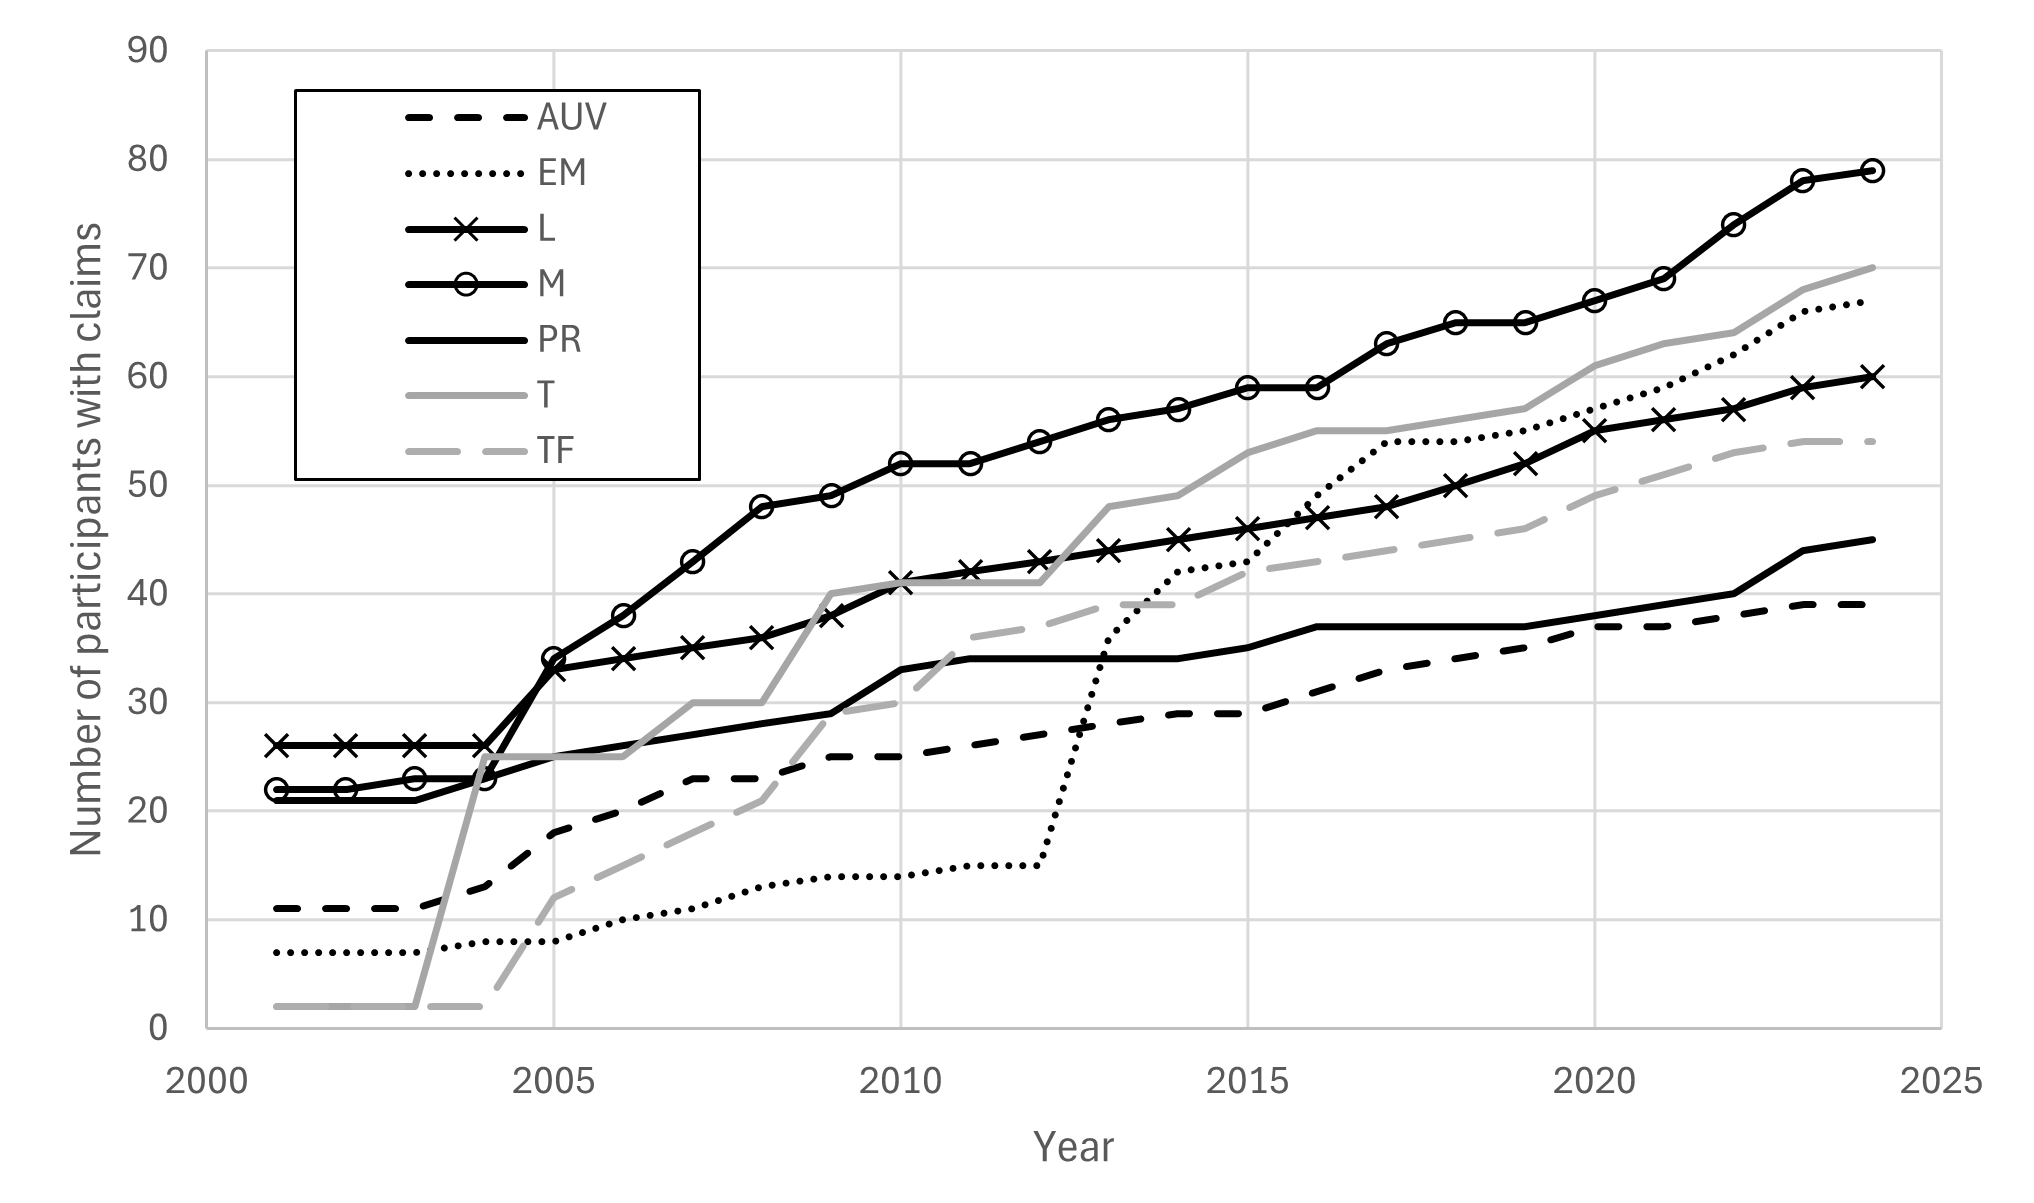
\includegraphics[width=\linewidth]{figures/Participants_Physics.png}
    \caption{Growth in the number of participants with at least one service in each of the Physics areas over time.}
    \label{fig:Physics_growth}
\end{figure}

Similar figures can be constructed for the branches of each Physics area as can be seen in the plots of figures \ref{fig:Branch_growth_a} and \ref{fig:Branch_growth_b}. Recall that we only accessed the history of services that were current in December 2024, so claims held and removed from the KCDB before that date are not visible in this dataset.

\begin{figure}
\centering
\begin{subfigure}[b]{0.48\textwidth}
    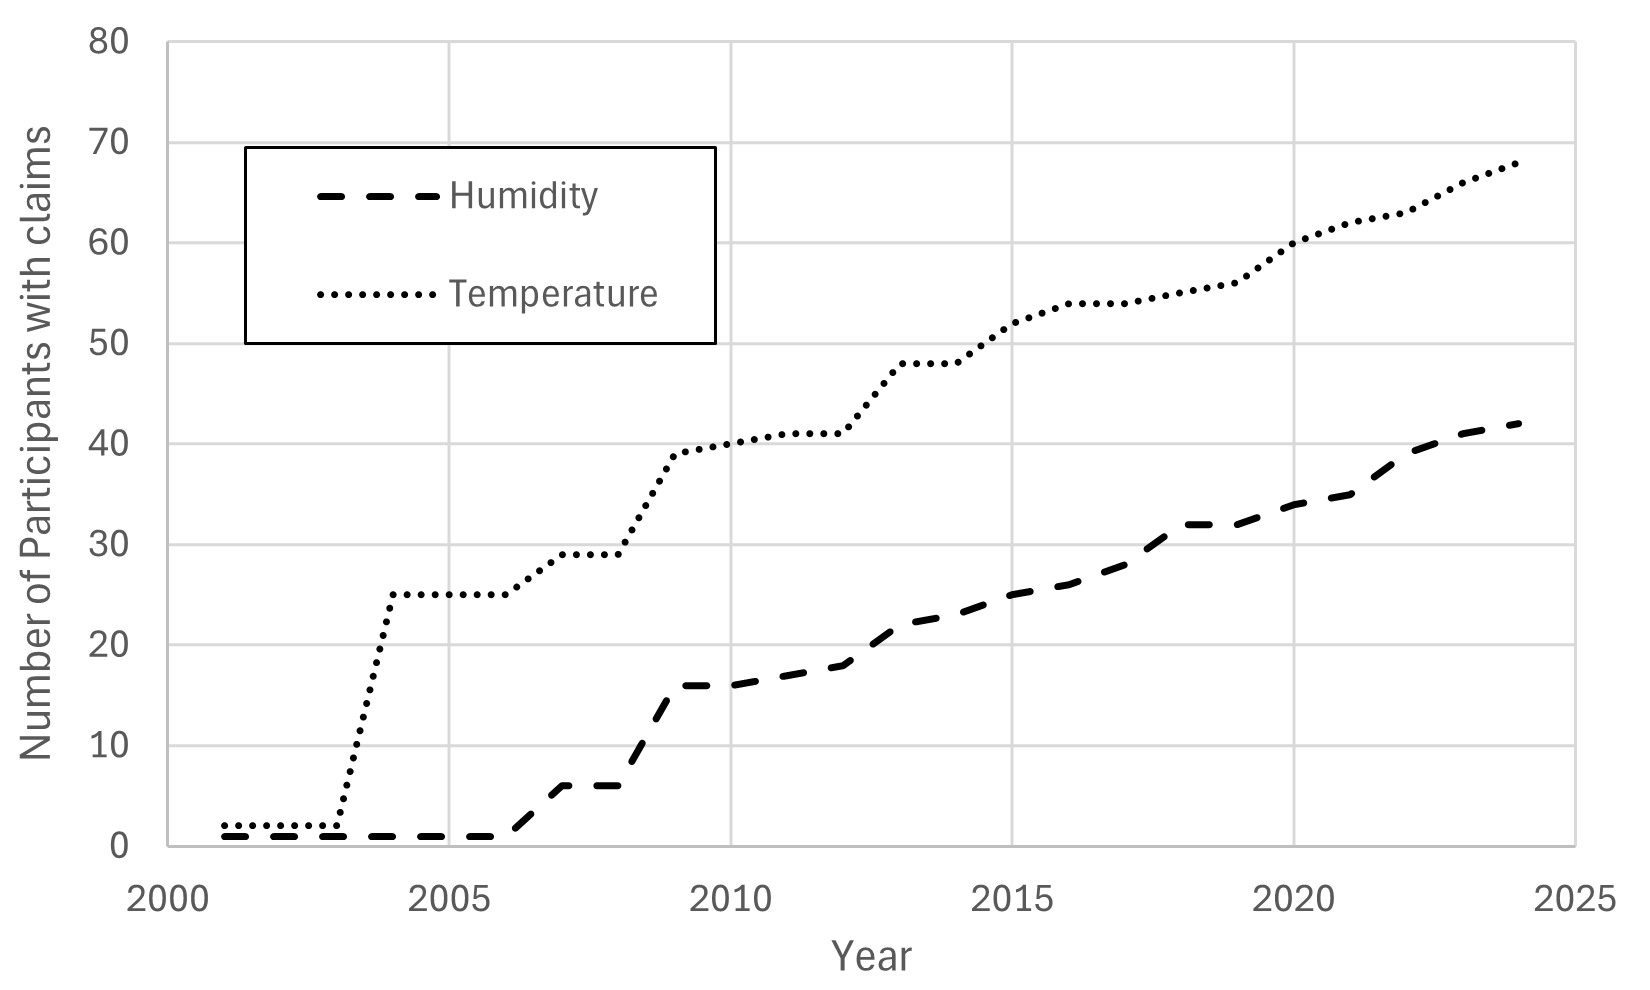
\includegraphics[width=\textwidth]{figures/Participants_Thermometry.png}
    \caption{Thermometry}
    \label{fig:t_vs_time}
\end{subfigure}
\hfill
\begin{subfigure}[b]{0.48\textwidth}
    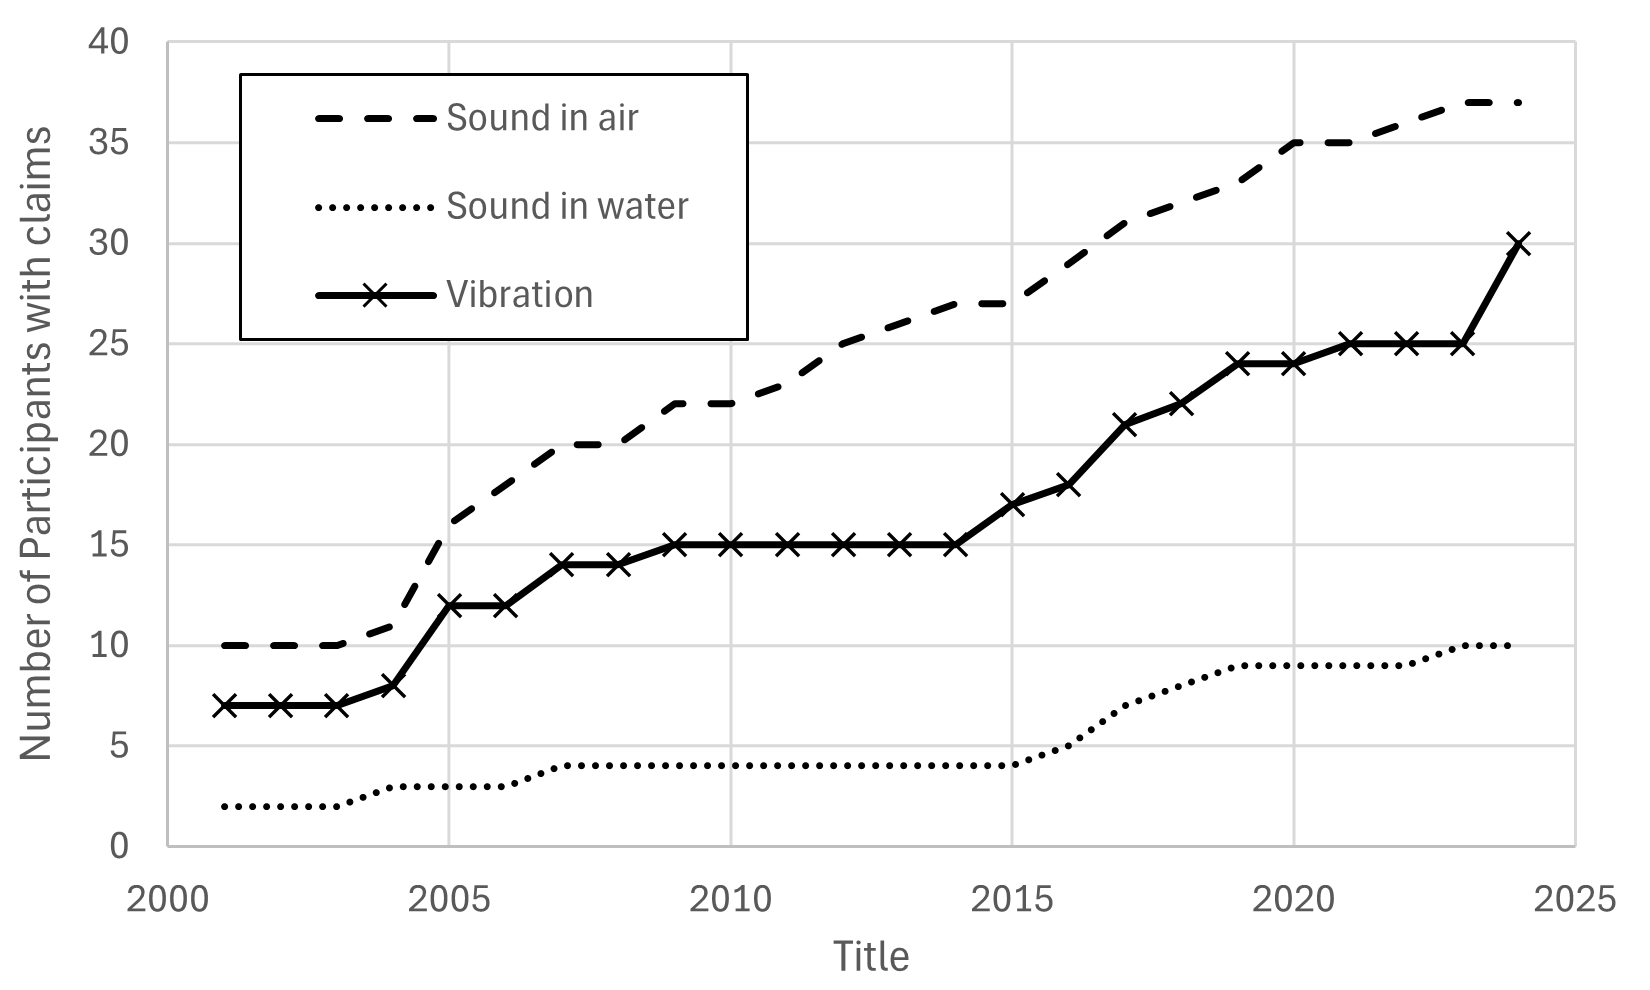
\includegraphics[width=\textwidth]{figures/Participants_Acoustics.png}
    \caption{Acoustics, Ultrasound and Vibration}
    \label{fig:auv_vs_time}
\end{subfigure}
\hfill
\begin{subfigure}[b]{0.48\textwidth}
    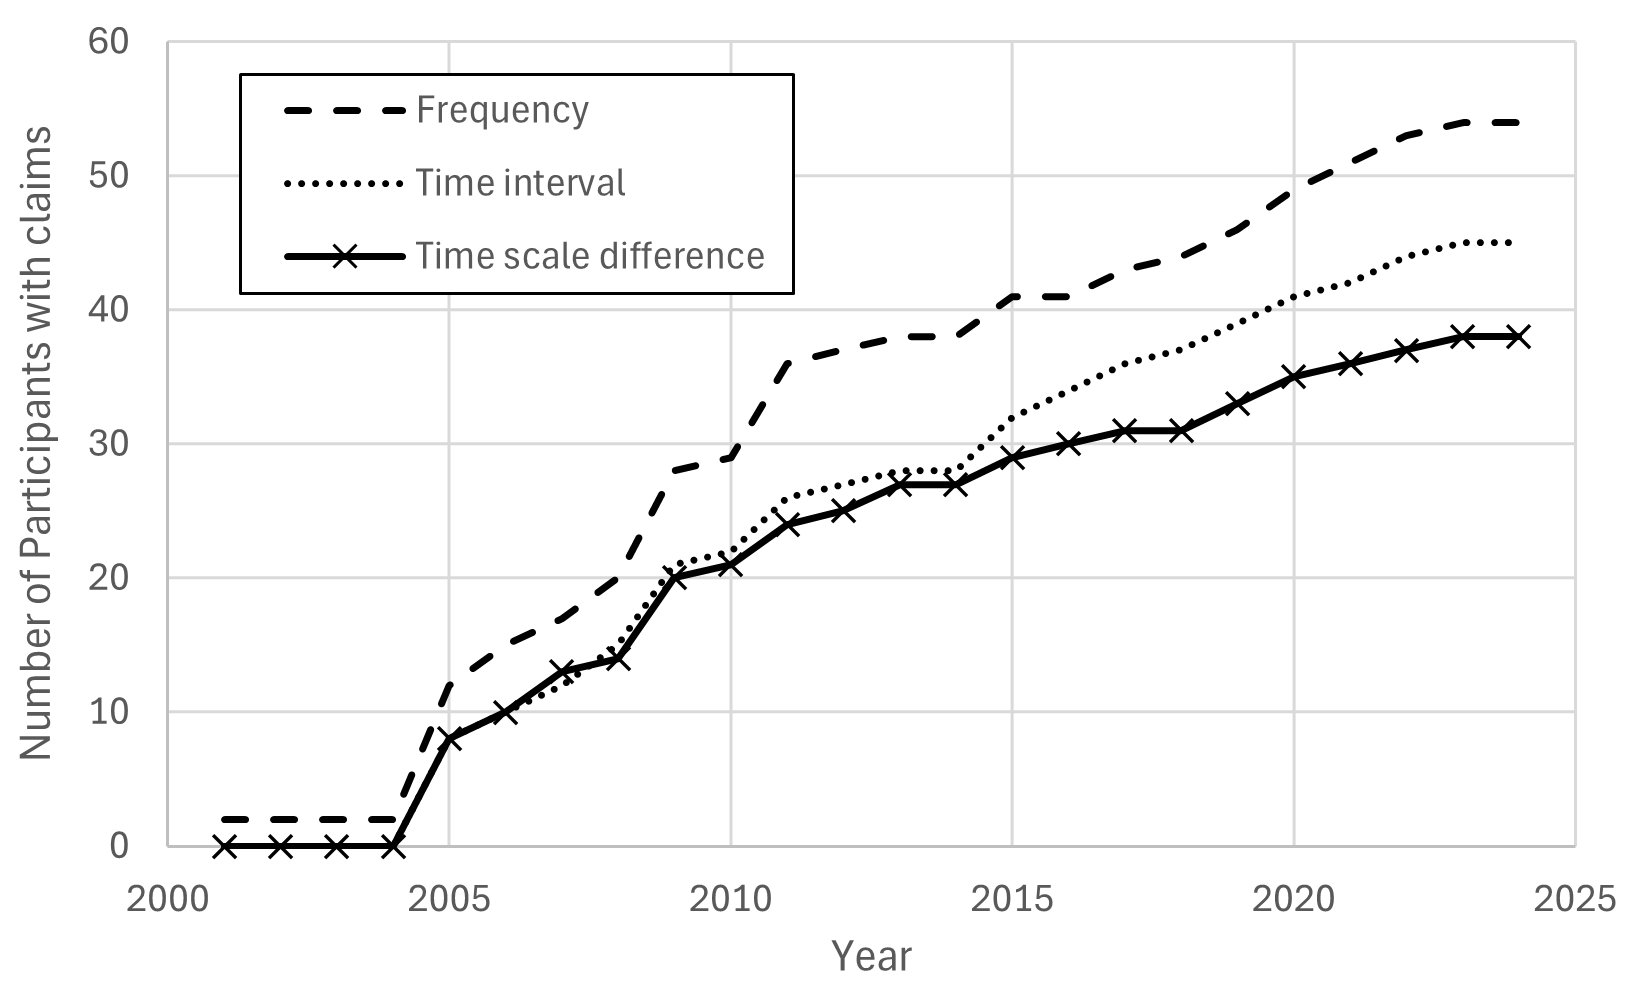
\includegraphics[width=\textwidth]{figures/Participants_Time.png}
    \caption{Time and Frequency}
    \label{fig:tf_vs_time}
\end{subfigure}
\hfill
\begin{subfigure}[b]{0.48\textwidth}
    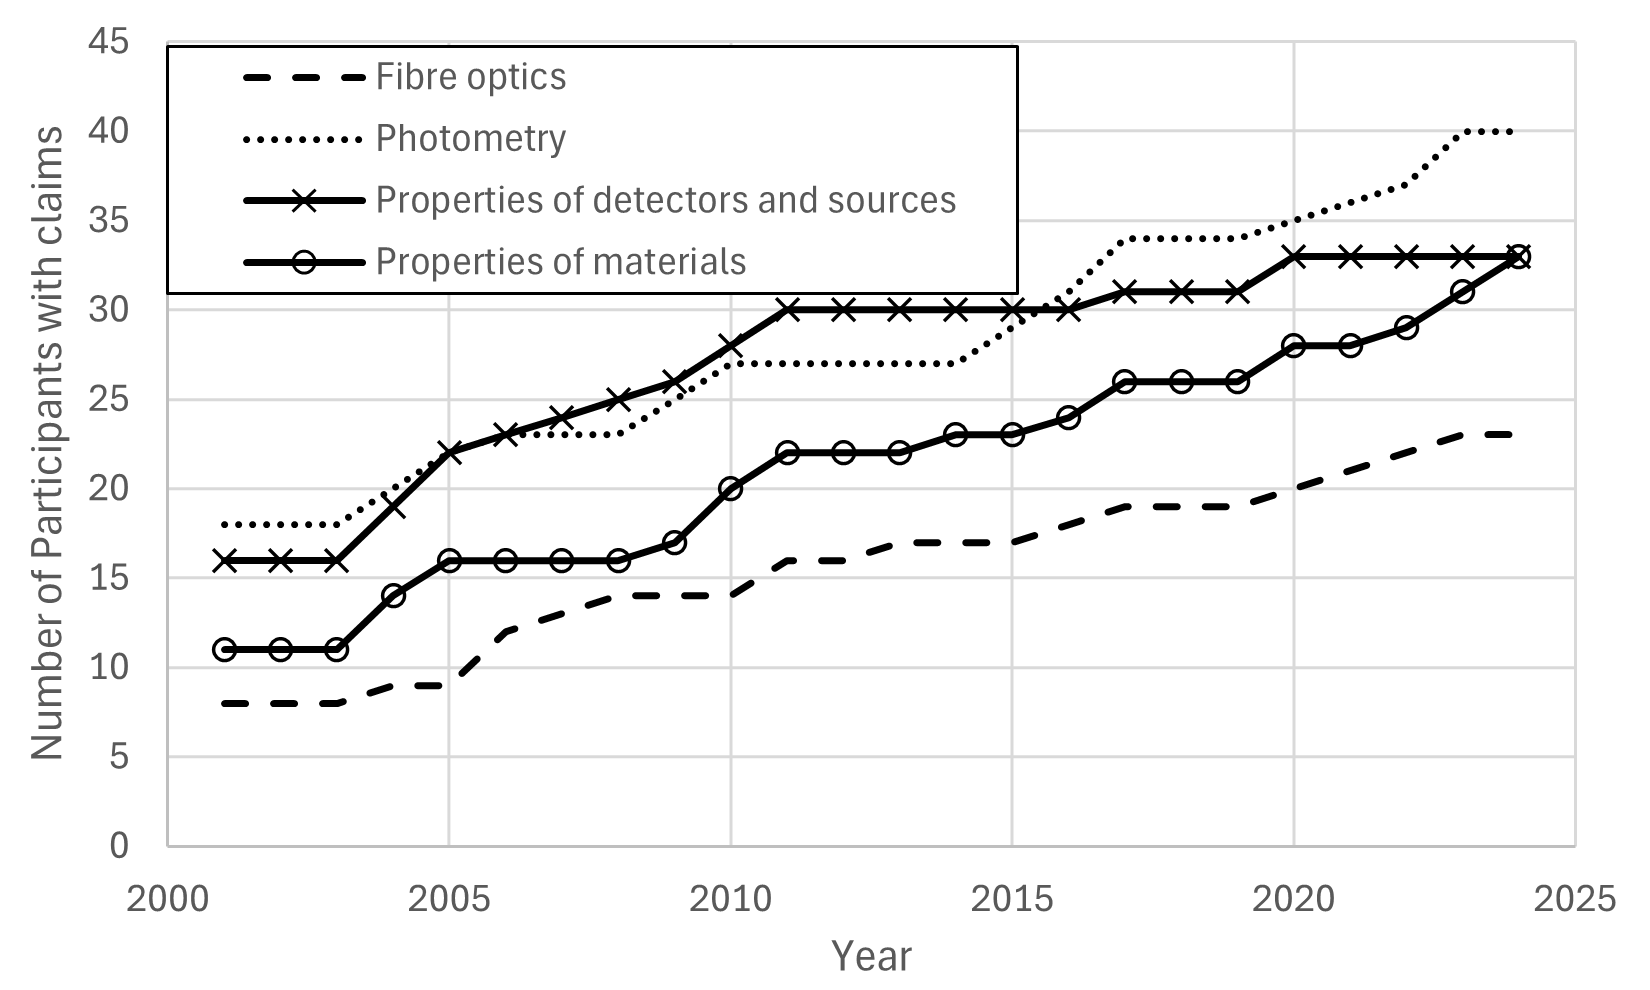
\includegraphics[width=\textwidth]{figures/Participants_Photometry.png}
    \caption{Photometry and Radiometry}
    \label{fig:pr_vs_time}
\end{subfigure}

\caption{The change in number of participants with claims in the KCDB for the (a) Thermometry, (b) Acoustics, Ultrasound and Vibration, (c) Time and Frequency, and, (d) Photometry and Radiometry branches with time.}
\label{fig:Branch_growth_a}
\end{figure}

\begin{figure}[!t]
\centering
\begin{subfigure}[b]{0.48\textwidth}
    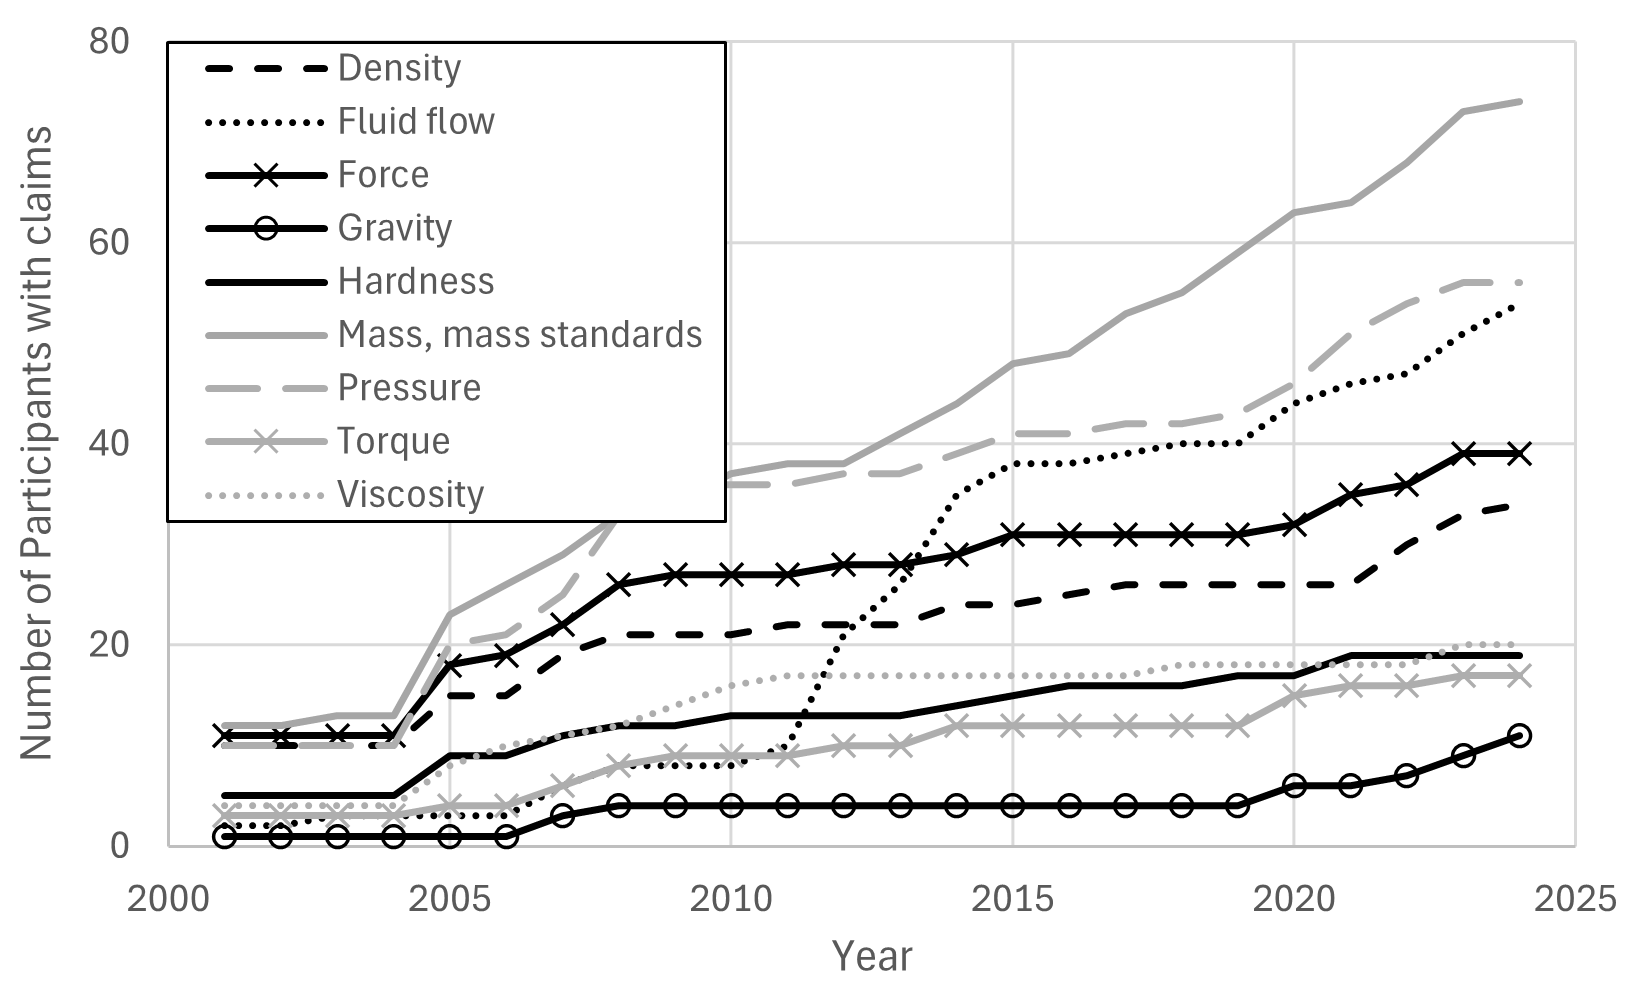
\includegraphics[width=\textwidth]{figures/Participants_Mass.png}
    \caption{Mass and Related Quantities}
    \label{fig:m_vs_time}
\end{subfigure}
\hfill
\begin{subfigure}[b]{0.48\textwidth}
    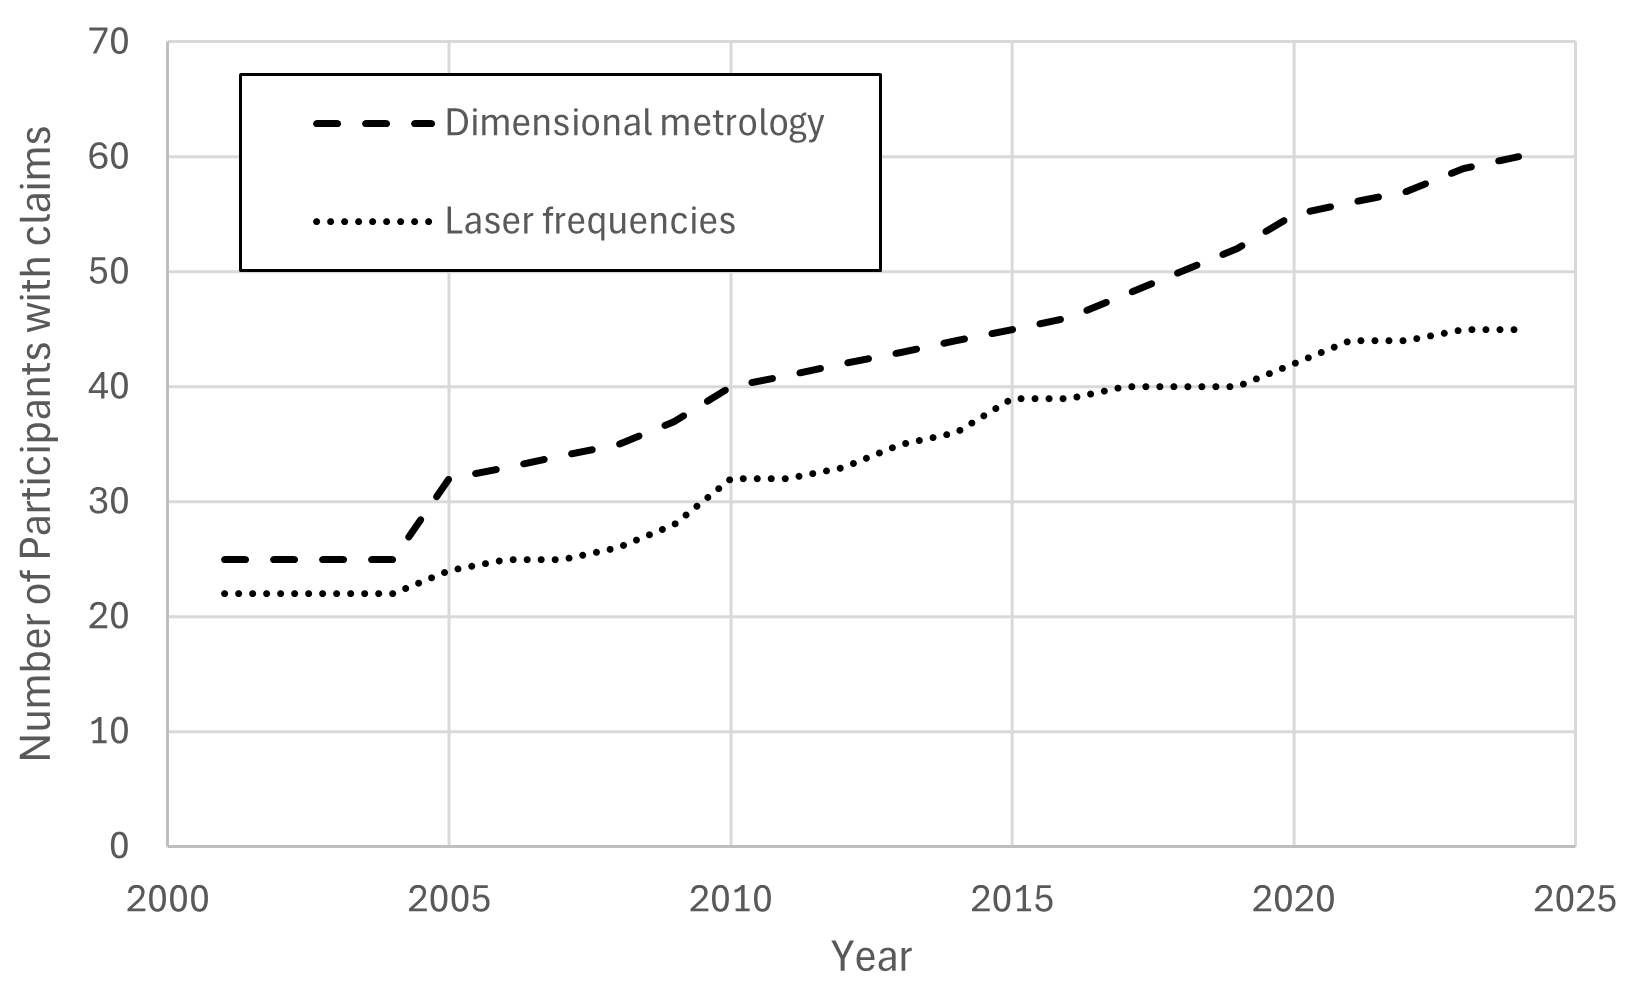
\includegraphics[width=\textwidth]{figures/Participants_Length.png}
    \caption{Length}
    \label{fig:l_vs_time}
\end{subfigure}
\hfill
\begin{subfigure}[b]{0.48\textwidth}
    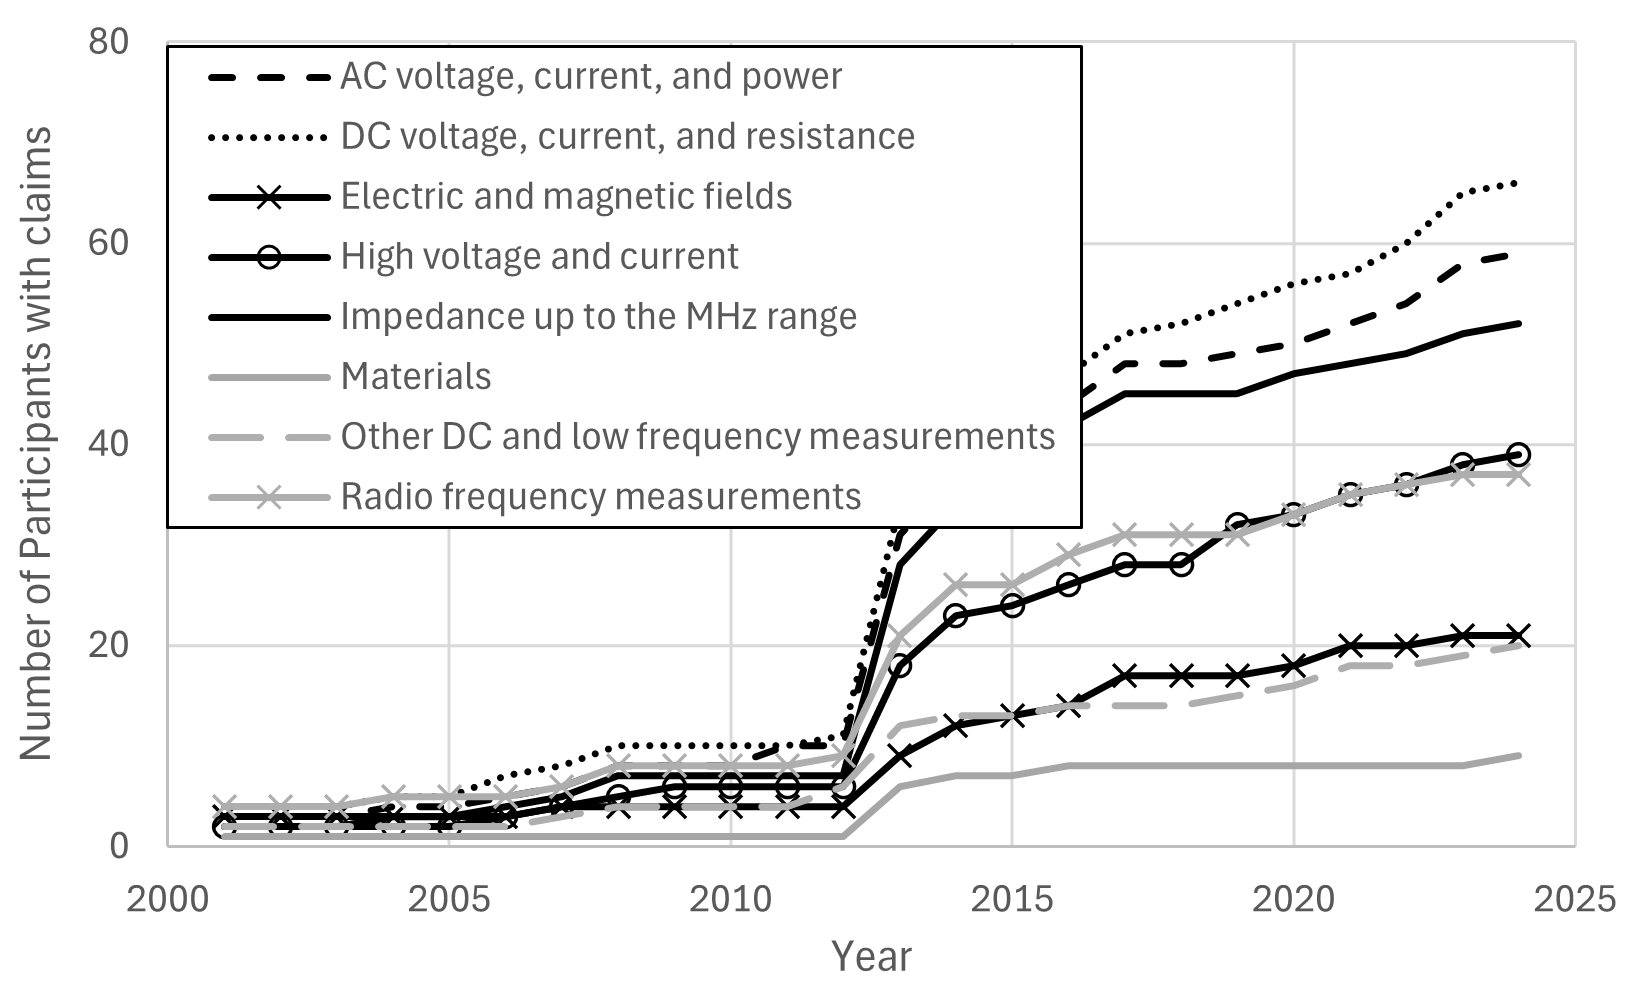
\includegraphics[width=\textwidth]{figures/Participants_Electrical.png}
    \caption{Electricity and Magnetism}
    \label{fig:em_vs_time}
\end{subfigure}

\caption{The change in number of participants with claims in the KCDB for the (a) Mass and Related Quantities, (b) Length, and, (c) Electricity and Magnetism branches with time.}
\label{fig:Branch_growth_b}
\end{figure}

\section{Discussion}

This view of the number of claims in the KCDB -- counted by the number of individual service categories claimed -- is presented as a more discerning measure than the simple raw number of CMCs as a way of understanding the range of services available within a State, Economy or international organisation. It is insensitive to situations where a participant may claim several CMCs within an individual service category due to variations in the uncertainty achievable as various parameters vary.

Like all simple metrics, this way of counting capability is also insensitive (like the raw number of CMCs also was) to the quality of a CMC -- to the level of uncertainty claimed, to the range of the measurand claimed, or to the dependent parameter range it is claimed over.

Access to this deeper level of comparison will become easier as the level of harmonisation of notation and expression of uncertainty claims in the KCDB increases. Many of the Consultative Committees are working on this with their members.

In the Chemistry and Biology, and Ionising Radiation domains of the KCDB, the 'free text' nature of some of the fields describing the services already impedes an analysis similar to the one carried out here for the Physics domain.


%----------------------------------------------------------------------------------------
%	 REFERENCES
%----------------------------------------------------------------------------------------
\printbibliography % Output the bibliography

%----------------------------------------------------------------------------------------



\end{document}
